\documentclass[12pt]{article}
%%% DOCUMENT FORMATTING %%%
\usepackage[margin=1in]{geometry}
\usepackage{enumitem}
\setlength{\parindent}{0pt}
\newcommand{\disp}{\displaystyle}

%%% HEADER %%%
\usepackage{fancyhdr}
\pagestyle{fancy}
\fancyhf{}
\lhead{MATH 1060}
\rhead{Vagnozzi}
\cfoot{\thepage}

%%% MATH NOTATION & SYMBOLS %%%
\usepackage{amssymb}
\usepackage{amsmath}
\newcommand{\R}{\mathbb{R}}
\newcommand{\N}{\mathbb{N}}
\newcommand{\Z}{\mathbb{Z}}
\newcommand{\lp}{\left(}
\newcommand{\rp}{\right)}
\newcommand{\ls}{\left[}
\newcommand{\rs}{\right]}
\newcommand{\lb}{\left\{}
\newcommand{\rb}{\right\}}
\newcommand{\arccot}{\text{arccot}}
\newcommand{\arccsc}{\text{arccsc}}
\newcommand{\arcsec}{\text{arcsec}} 

%%% TABLES %%%
\usepackage{colortbl}

%%% GRAPHS %%%
\usepackage{tikz}
\usepackage{pgfplots}
\pgfplotsset{compat=1.15}
\usepgfplotslibrary{fillbetween}
\usetikzlibrary{angles,quotes}

%%% ENVIRONMENTS %%%
\newcommand{\Example}{\paragraph{\Writinghand \hspace{0.1mm} Example.}}
\newcommand{\ExampleCont}{\paragraph{\Writinghand \hspace{0.1mm} Example (continued).}}
\newcommand{\boxenv}[2]{
	\fbox{
	\begin{minipage}{0.97\textwidth}
	\vspace{2mm}	
	\paragraph{#1} #2
	\vspace{2mm}
	\end{minipage}
	}}

%%% FUN THINGS %%%
\newcommand*\tc[1]{\tikz[baseline=(char.base)]{
            \node[shape=circle,draw,inner sep=2pt] (char) {#1};}}
\usepackage{marvosym}

%%% MISC %%%
\usepackage{hyperref}


\setcounter{page}{115}

\begin{document}
\section*{4.2: Mean Value and Rolle's Theorems}

\boxenv{Learning Objectives.}{Upon successful completion of Section 4.2, you will be able to\dots
		
	\begin{itemize}[leftmargin=6mm]
		\item Answer conceptual questions involving Rolle's Theorem and the Mean Value Theorem.
		\item Determine if Rolle's Theorem applies and find the point(s) guaranteed to exist by Rolle's Theorem.
		\item Find the point(s) guaranteed to exist by the Mean Value Theorem.
		\item Find functions with the same derivative of a given function.
		\item Use graphs to answer questions involving the Mean Value Theorem.
		\item Solve applications involving the Mean Value Theorem.
	\end{itemize}
	\vspace{-4mm}
}

\vspace{5mm}

\subsection*{Rolle's Theorem}

How can we determine whether a function has a zero derivative? Rolle's Theorem is a useful result of calculus that allows us to guarantee the existence of at least one horizontal tangent line if certain conditions hold.

\vspace{5mm}

\boxenv{Rolle's Theorem.}{If $f$ is a function that is
\vspace{2mm}
\begin{enumerate}
\item[\tc{1}] continuous on $[a,b]$,
\item[\tc{2}] differentiable on $(a,b)$, and
\item[\tc{3}] $f(a)=f(b)$,
\end{enumerate}
then there exists at least one $c\in (a,b)$ such that $f'(c)=0$.
}

\vspace{2mm}

 \begin{center}
            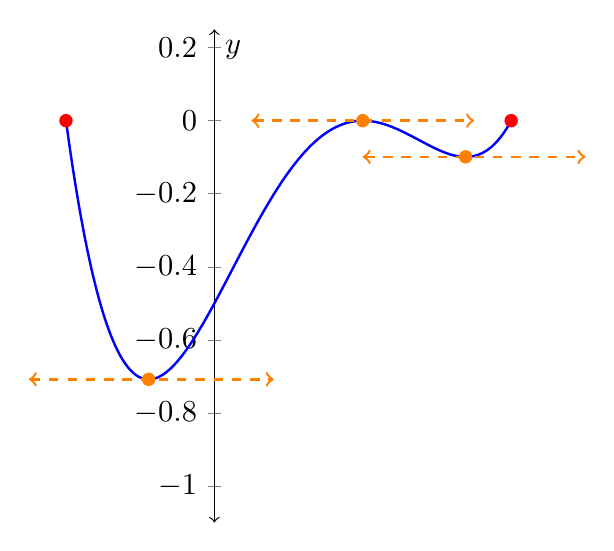
\begin{tikzpicture}[scale=1.1]
                \begin{axis}[
                	axis x line=none,
                	xmax=2.5, xmin=-1.5,
                	axis y line=center,
                	ymax=0.25, ymin=-1.1,
                	xlabel=$x$,ylabel=$y$,
                	axis line style = {<->}
                    ]
                    \addplot[name path=f,smooth,domain=-1:2,color=blue,samples=100,thick] {0.25*x^4 - 0.75*x^3 + 0.25*x^2 + 0.75*x - 0.5};
                    \addplot[name path=f,smooth,domain=-1.25:0.40,color=orange,dashed,samples=100,<->,thick] {-0.708};
		    \addplot[mark=*,color=red] coordinates {(-1,0)};
		    \addplot[mark=*,color=red] coordinates {(2,0)};
		    \addplot[mark=*,color=orange] coordinates {(-0.443,-0.708)};
		    \addplot[mark=*,color=orange] coordinates {(1.693,-0.099)};
		    \addplot[mark=*,color=orange] coordinates {(1,0)};
                    \addplot[name path=f,smooth,domain=1:2.5,color=orange,dashed,samples=100,<->,thick] {-0.099};
                    \addplot[name path=f,smooth,domain=0.25:1.75,color=orange,dashed,samples=100,<->,thick] {0};
                \end{axis}
            \end{tikzpicture}
        \end{center}
        
        \newpage
        
        The following functions are continuous on their domains, which is a fact you can cite when making Rolle's Theorem arguments.
        \begin{itemize}
        	\item Polynomials
        	\item Rational Functions
        	\item Root Functions
        	\item Trig and Inverse Trig Functions
        	\item Exponential Functions
        	\item Logarithmic Functions
        \end{itemize}
    
    \vspace{3mm}
        
        \Example Consider $f(x)=\sin(2x)$ on $\disp\ls 0,\frac{\pi}{2}\rs$.
        
        \begin{enumerate}
        \item[\tc{1}] Verify that Rolle's Theorem applies.
        
        \vspace{55mm}
        
        \item[\tc{2}] Find all points $c$ guaranteed to exist by the theorem.
        \end{enumerate}

\newpage
        
\subsection*{Mean Value Theorem}

Rolle's Theorem is a special case of a more general theorem known as Mean Value Theorem.

\vspace{5mm}

\boxenv{Mean Value Theorem (MVT).}{If $f$ is a function that is

\vspace{2mm}
\begin{enumerate}
\item[\tc{1}] continuous on $\ls a,b\rs$ and
\item[\tc{2}] differentiable on $(a,b)$, 
\end{enumerate}
then there exists at least one point $c\in (a,b)$ such that
$$f'(c)=\frac{f(b)-f(a)}{b-a}.$$

\vspace{-4mm}}

\vspace{5mm}

The Mean Value Theorem guarantees that there is a point $c$ where the slope of the tangent line at $c$ matches the slope of the secant line through the endpoints of the closed interval.

\begin{center}
            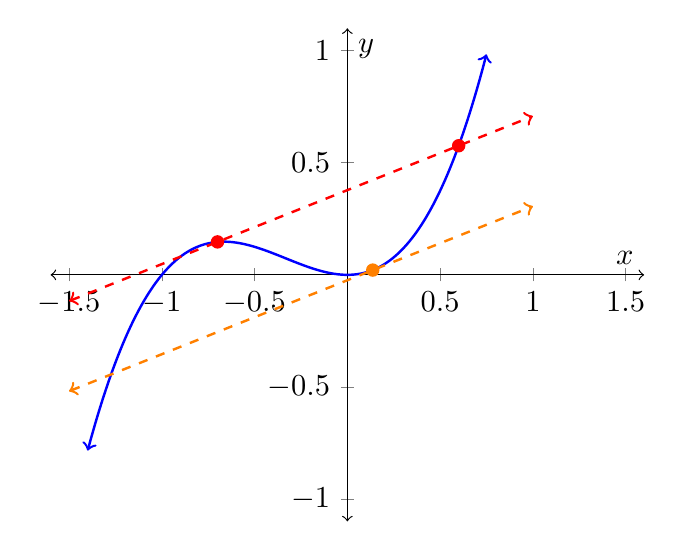
\begin{tikzpicture}[scale=1.1]
                \begin{axis}[
                	axis x line=middle,
                	xmax=1.6, xmin=-1.6,
                	axis y line=center,
                	ymax=1.1, ymin=-1.1,
                	xlabel=$x$,ylabel=$y$,
                	axis line style = {<->}
                    ]
                    \addplot[name path=f,smooth,domain=-1.4:0.75,color=blue,samples=100,<->,thick] {x^3 + x^2};
                    \addplot[name path=f,smooth,domain=-1.5:1,color=red,dashed,samples=100,<->,thick] {0.33*x + 0.378};
                    \addplot[name path=f,smooth,domain=-1.5:1,color=orange,dashed,samples=100,<->,thick] {0.33*x - 0.024};
		    \addplot[mark=*,color=red] coordinates {(-0.7,0.147)};
		    \addplot[mark=*,color=red] coordinates {(0.6,0.576)};
		    \addplot[mark=*,color=orange] coordinates {(0.1369,0.0213)};
                \end{axis}
            \end{tikzpicture}
        \end{center}
        
\vspace{3mm}

Let's further explore the connection between the MVT and Rolle's.
\vspace{2mm}

\begin{center}
\begin{tikzpicture}[scale=1.1]
                \begin{axis}[
                	axis x line=middle,
                	xmax=1.6, xmin=-1.6,
                	axis y line=center,
                	ymax=1.1, ymin=-1.1,
                	xlabel=$x$,ylabel=$y$,
                	axis line style = {<->}
                    ]
                \end{axis}
            \end{tikzpicture} 
\end{center}

\newpage

\Example Consider $f(x)=\sqrt{4-x^2}$ on the interval $[0,2]$. 

\begin{itemize}
\item[\tc{1}] Verify that the MVT applies to $f$ on this interval.

\vspace{50mm}

\item[\tc{2}] Find all points $c$ guaranteed to exist by the theorem.

\vspace{50mm}

\end{itemize}

\Example You enter a six-mile-long stretch of toll road at 1:30 PM and exit at 1:35~PM with no stops in between. Suppose that the road does not have any bends and that the toll road has a speed limit of 65 mph. Two weeks later, you get a speeding ticket in the mail. How can the toll authority prove you were speeding?
\end{document}